\section{Implementation of Model-view-controller}
In Figure \vref{fig:overview} is an overview how our model-view controller architecture has been implemented in our application where the arrows are call dependencies. It is an incomplete representation for the GIRAFAdmin because not all classes have been included in the figure, however, all the connections between the controller and model's classes are represented. 

In the figure the Model's seven classes, \emph{sql\_helper} excluded, are all used by at least one controller while the \emph{sql\_helper} is used by the other classes to relay SQL commands to the database. The model will be further explained in section \vref{model}. All in all six views have been implemented (header, footer and four pure "content" views) with the functions of login, main site view and the contact book's functionality. The views will be explained further in section \vref{view}. Likewise, eight controllers have been implemented, the purpose of which will be explained in section \vref{controller}.

\begin{figure}
	\centering
		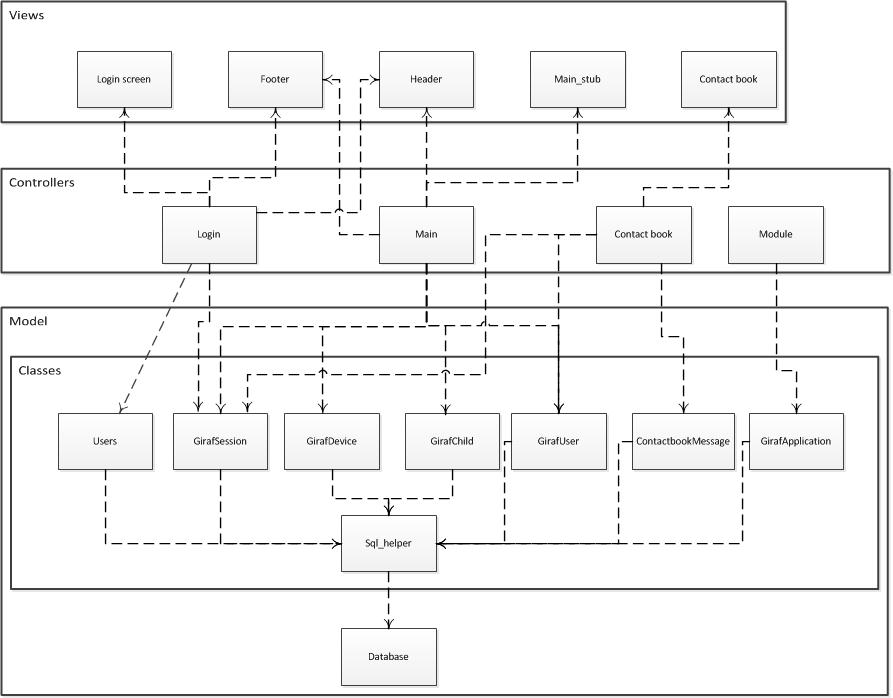
\includegraphics[width=1.00\textwidth]{img/overview.jpg}
	\caption{model-view-controller overview}
	\label{fig:overview}
\end{figure}
